\section{Materials and blueprints}

\subsection{Floating platform}

The floating platform is built up from the following parts:

\begin{itemize}
  \item 1 main plate made  from 22~mm thick glulam wood. Observe that in the
    blueprint for this plate holes for cables, and screw holes for the
    propeller holder and circuit boards are not included. The front bumper,
    servo and containing straps for the batteries are screwed to this plate.(Fig.~\ref{fig:appendix-blueprint-main-plate})
  \item 4 floating elements made from 70~mm XPS cell foam (Fig. \ref{fig:appendix-blueprint-ponton})
  \item 2 boards that goes below the floating elements (Fig. \ref{fig:appendix-blueprint-ponton})
  \item 4 250~mm M10 stainless steel threaded rods
  \item 8 70~mm M6 stainless steel threaded rods
  \item 4 M10 nuts
  \item 4 M10 lock nuts
  \item 16 M6 nuts
  \item 8 M6 wing nuts
  \item 8 M10 washers
  \item A 20~mm plastic tube bent to a quarter circle with a radius of 403~mm,
    with 100~mm extra material to attach in each end.
  \item 2 straps to keep the batteries in place
  \item 4 carry handles
  \item Self drilling screws, and washers used to attach electronics, battery
    straps, and bumper.
  \end{itemize}

  \begin{figure}
    \centering
    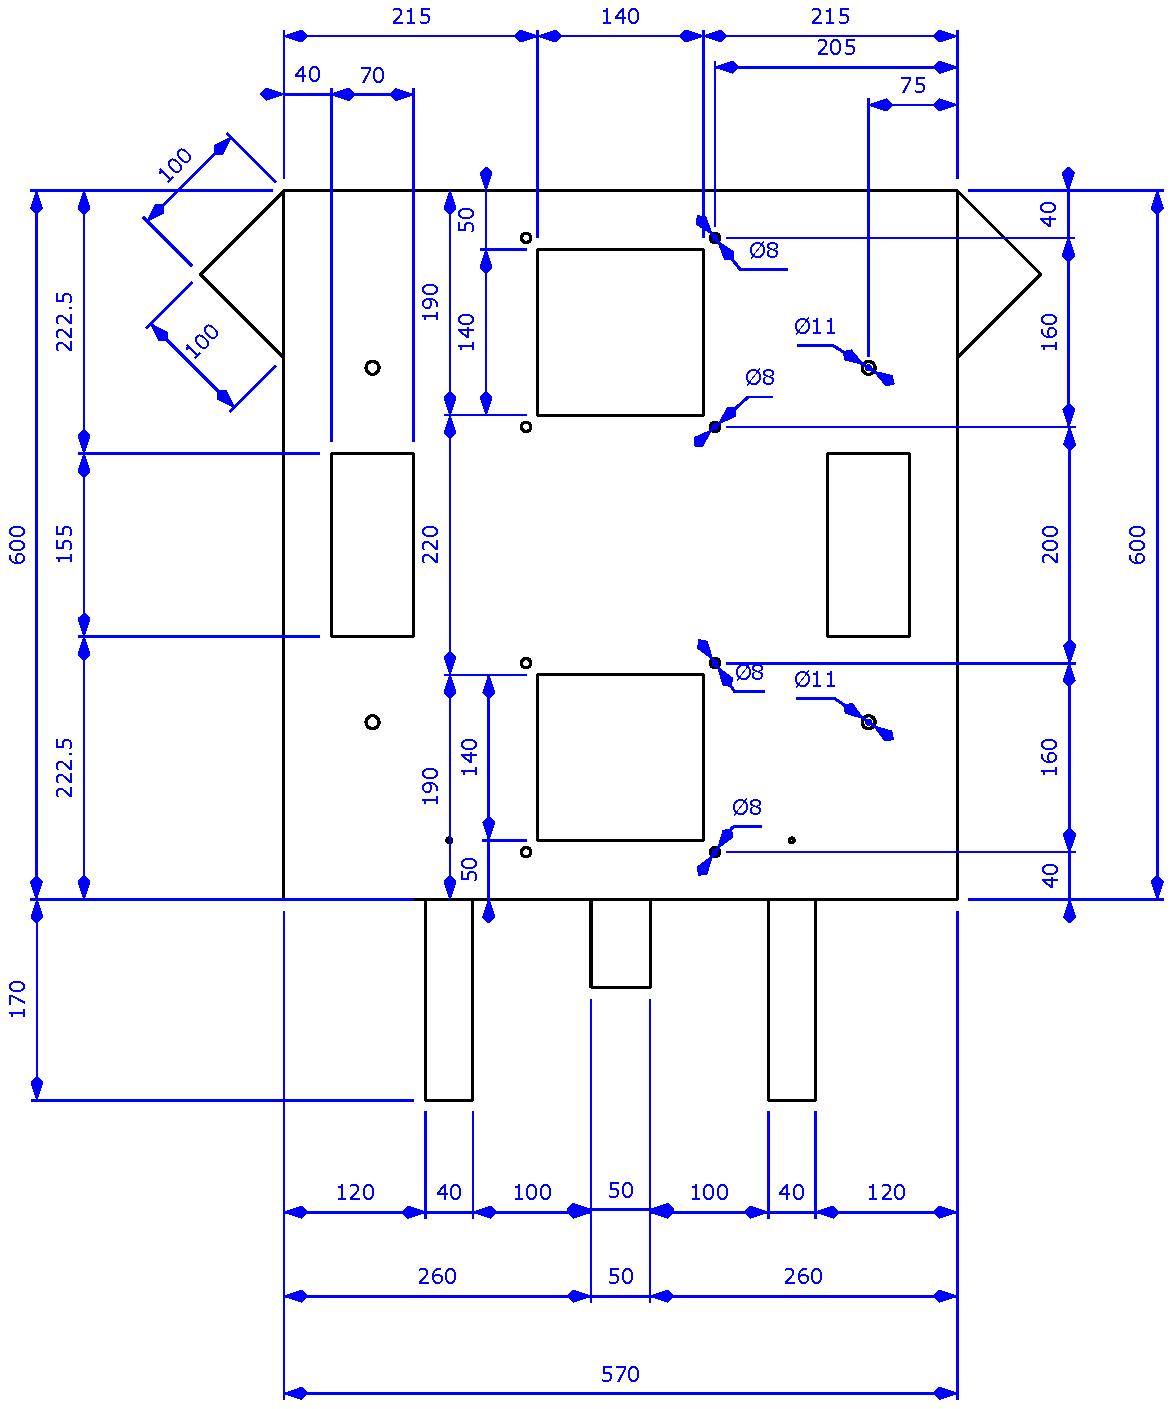
\includegraphics[scale=0.5]{mainPlate}

    \caption{The bluprint of the main plate in scale 1:10}
    \label{fig:appendix-blueprint-main-plate}
\end{figure}


  \begin{figure}
    \centering

    \raisebox{-\height}{ 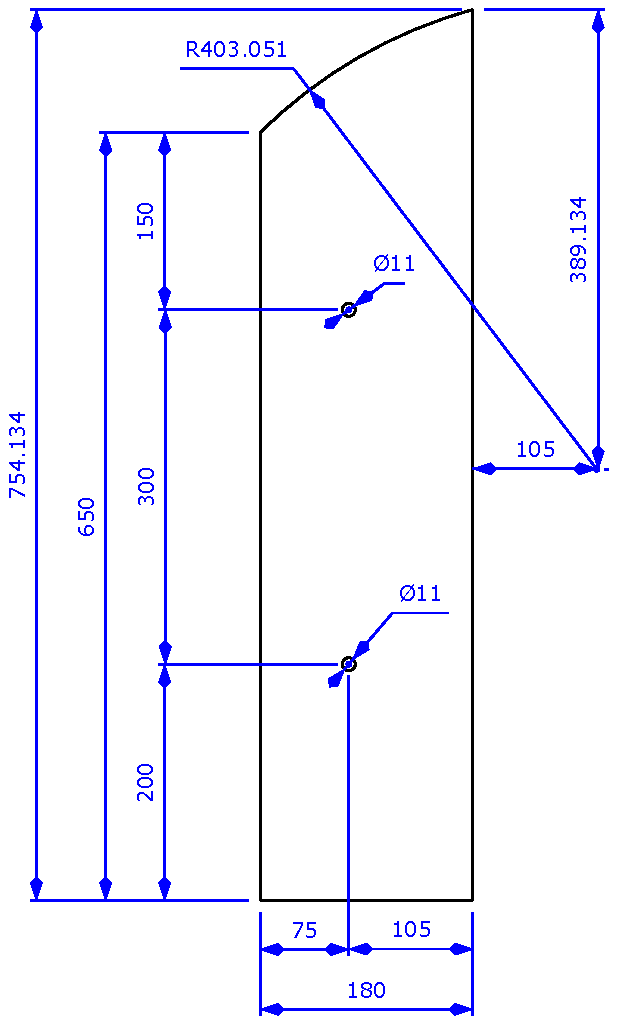
\includegraphics[scale=0.5]{ponton}}
    \raisebox{-1.1\height}{ 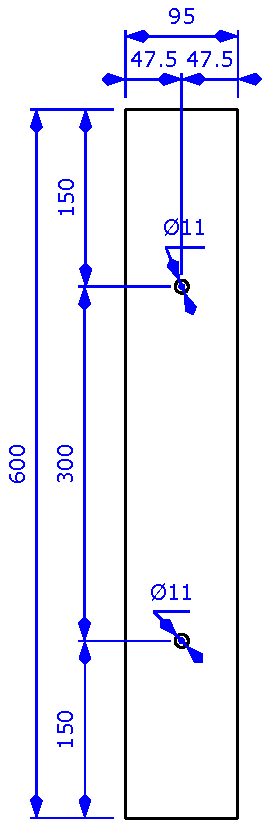
\includegraphics[scale=0.5]{bottom_plank}}
   
    \caption{The bluprint of one ponton and the bottom board in scale 1:10}
    \label{fig:appendix-blueprint-ponton}
\end{figure}
\subsection{Electronics}

The electronic components mounted on the platform are:

\begin{itemize}
  \item 1 Arduino Leonardo
  \item 1 Dual VNH5019 Motor Driver Shield
  \item 2 2725 Brushless Outrunner Motors 1600kv
  \item 2 ESC who matches the brushless motors
  \item 2 plastic propellers
  \item 1 15~kg servo
  \item 1 R9D Radio Control Receiver
  \item 1 blue power-LED (mounted on the cover)
  \item 1 220~$\Omega$ resistor
  \item 1 power switch (mounted on the cover)
  \item 1 0.1 $\mu$F capacitor rated for at least 12V \footnote{\label{fotnot_app} These items can be replaced with a pre built 12~V to 5~V power supply. The electronics are connected according to the circuit diagrams, and the files in \texttt{RBR\_driver.zip} is loaded onto the Arduino.} %\textsuperscript{\ref{fotnot_app}}%\footnotemark[1] 
  \item 1 22 $\mu$F capacitor rated for at least 5V \textsuperscript{\ref{fotnot_app}}
  \item 1 L4940V5 linear regulator \textsuperscript{\ref{fotnot_app}}%\footnotemark[1]
  \item Protoboard to build the 5~V PSU on \textsuperscript{\ref{fotnot_app}} \todo{insert circuit diagram reference in footnote}
     %\footnotemark[1] 
  \item A few meter mains cable 2x1.50~mm$^2$ unshielded
  \item A few meter signal cable
  \item A few sensor cables and connectors (for servo, ESC, and power to RC receiver) 
  \item Heatshrink tubing to cover connections
  \item A few blade receptacle 4.8x0.5~mm fully insulated, blade terminal red
    4.8x0.8~mm, ring cable lug 4.3~mm used to connect the cables together.
  \item A few 2.54~mm pin headers for the connections to the Arduino.
\end{itemize}
 Figure~\ref{fig:appendix-circuit-diagrams} shows the complete circuit diagram of these parts.

\begin{figure}[htbp]
  \centering
  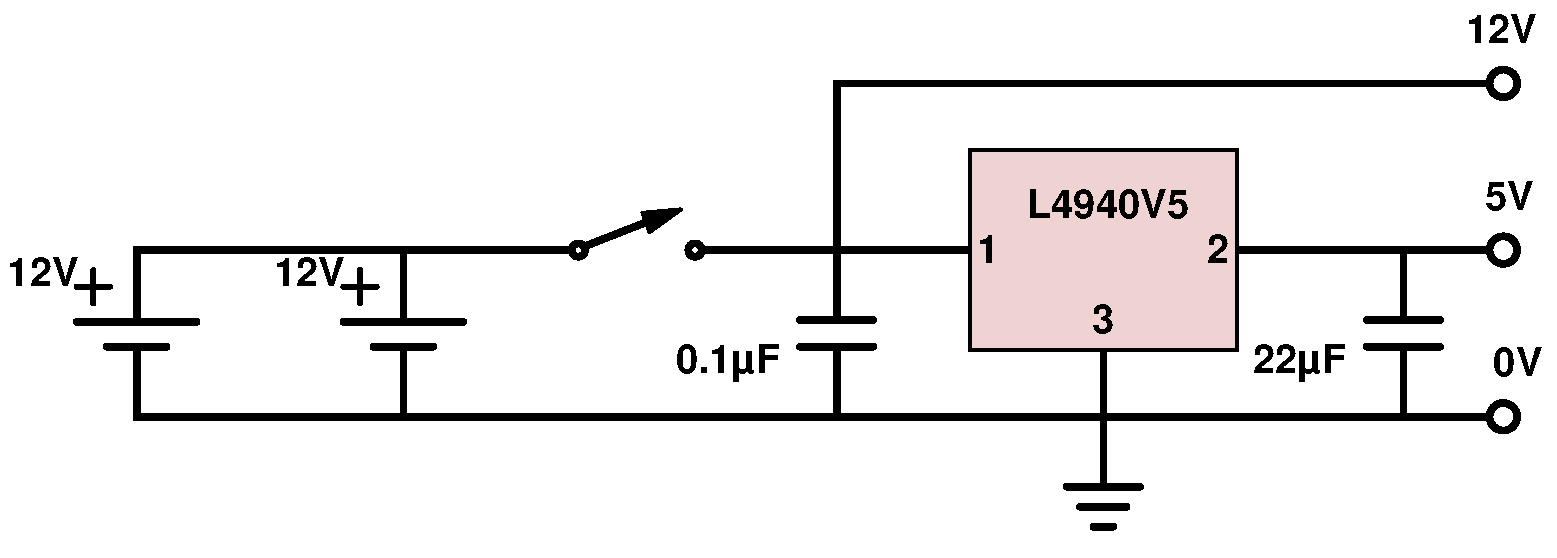
\includegraphics[width=0.7\textwidth]{Powersupply}
  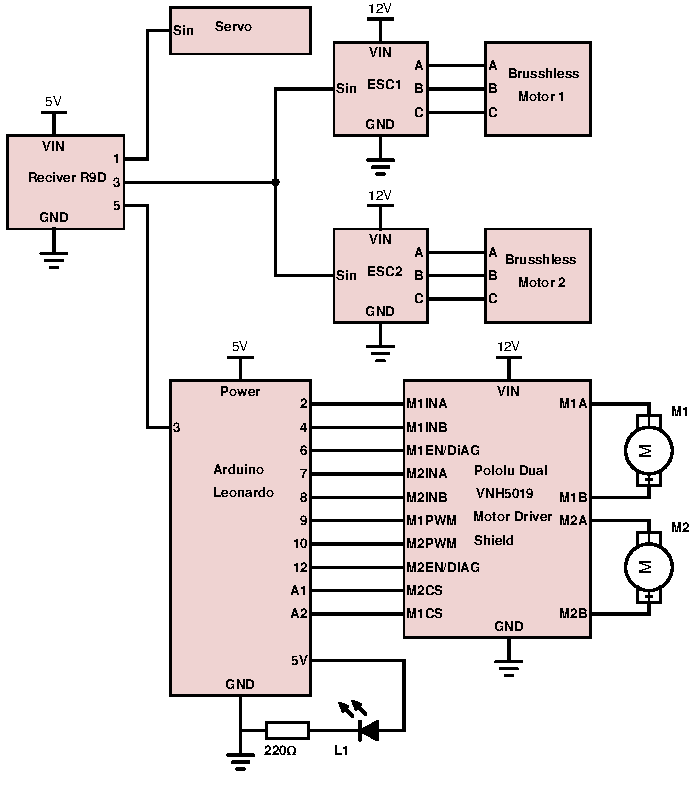
\includegraphics[width=0.7\textwidth]{circuit}
  
  \caption{The Circut Diagram for the electronics.}
  \label{fig:appendix-circuit-diagrams}
    
\end{figure}
%Note that the items marked with (*) can be replaced with a pre built 12~V to
%5~V power supply.  The electronics are connected according to the circuit
%diagrams, and the files in RBR\_driver.zip is loaded onto the Arduino.

\subsection{RBR modules}

Each of the two RBR modules are built up from:

\begin{itemize}
  \item 1 top plate made from a 22~mm thick board (observe that the holes for
    the 3D printed motor holder are not included.) (Fig. \ref{fig:appendix-blueprint-rbr-module})
  \item 1 bottom plate made from a 22~mm thick board (Fig. \ref{fig:appendix-blueprint-rbr-module})
  \item 1 3D printed motor holder
  \item 1 motor, shuck, and gearbox taken from a $\dots$
    screwdriver.\todo{Insert model here}
  \item 3 330~mm M10 stainless steel threaded rods
  \item 3 M10 locking nuts
  \item 9 M10 nuts
  \item 12 M10 washers
  \item 2 50~mm M4 stainless steel threaded rods
  \item 2 110~mm M4 stainless steel threaded rods
  \item 10 M4 washers
  \item 10 M4 nuts
  \item 4 long M3 screws
  \item 4 M3 nuts
  \item 4 M3 washers
  \item 1 shaft guide NS29
  \item 1 piece of 50~mm wide and 200~mm long piece of 2~mm stainless steel
    bent to form a baffle.
  \item 1 piece of metal to put pressure on top of the motor.
\end{itemize}


\begin{figure}[htbp]
  \centering
   \raisebox{-\height}{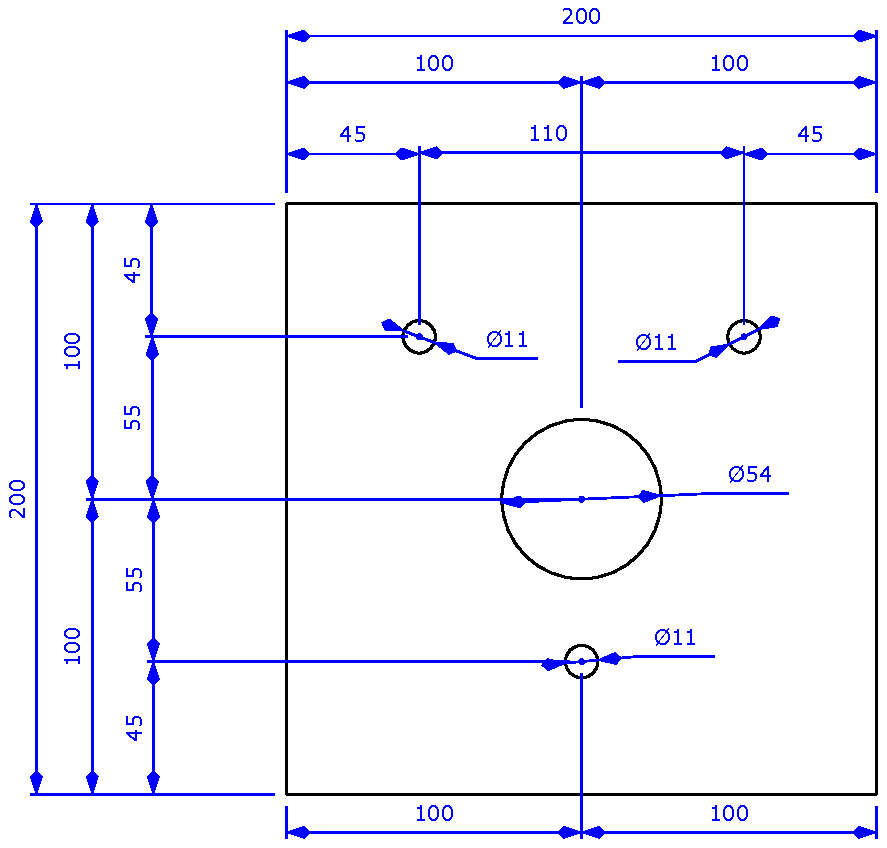
\includegraphics[scale=0.4]{RBR_mod_Top}}
   \raisebox{-1.02\height}{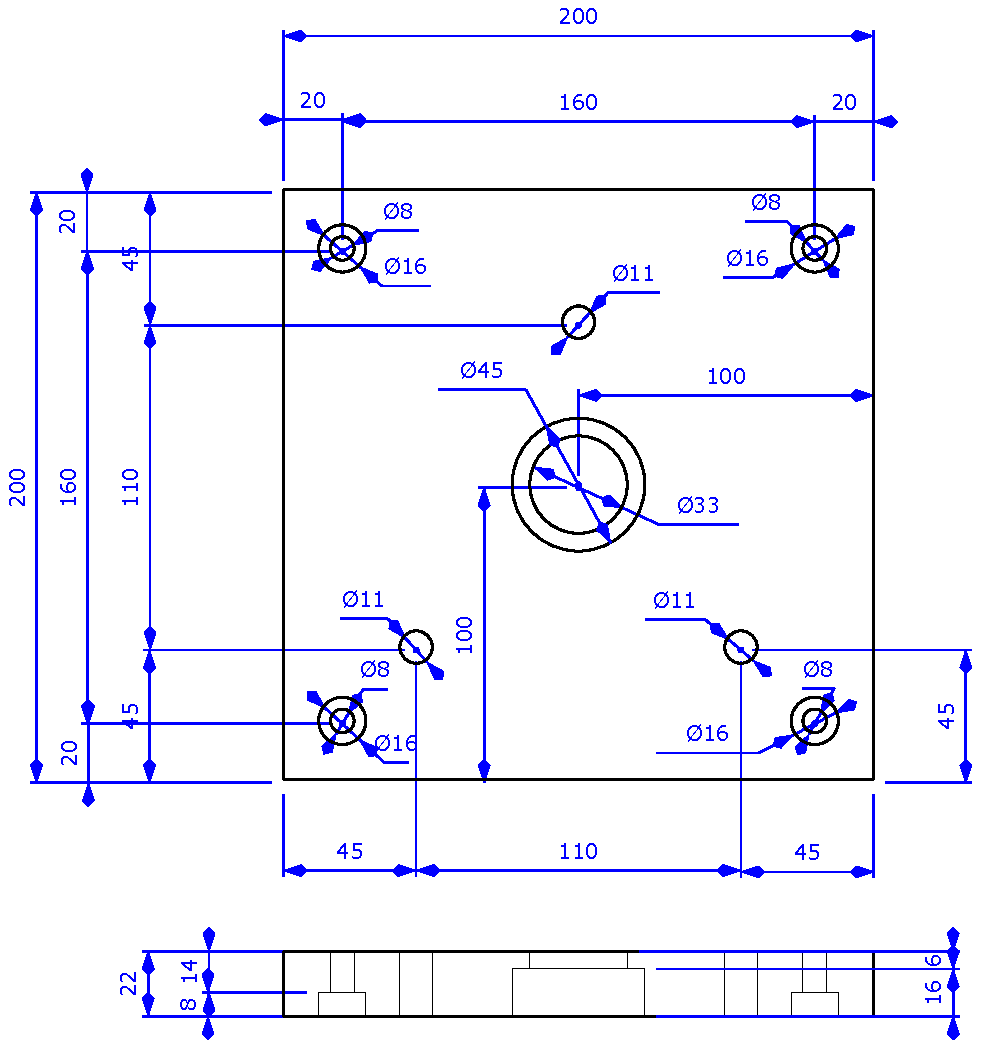
\includegraphics[scale=0.4]{RBR_mod_Bottom}}
  \caption{The top and bottom plates of the RBR module in scale 1:5}
  \label{fig:appendix-blueprint-rbr-module}
    
\end{figure}
\subsection{Covers for RBR modules and electronics}

The cover for the RBR module are made from 5 pieces of 3~mm thick acrylic glass
glued together, with a handle attached on top. The blueprints for these is shown in figures~\ref{fig:appendix-blueprint-rbr-cover} and \ref{fig:appendix-blueprint-electronic-cover}.

The cover for the electronics are made from 13 pieces of 3~mm thick acrylic glass
glued together. On top of this cover the power switch is connected. This cover
was fastened to the platform using handmade angle brackets and a nut.

\begin{figure}[htbp]
  \centering
 \raisebox{-\height}{ 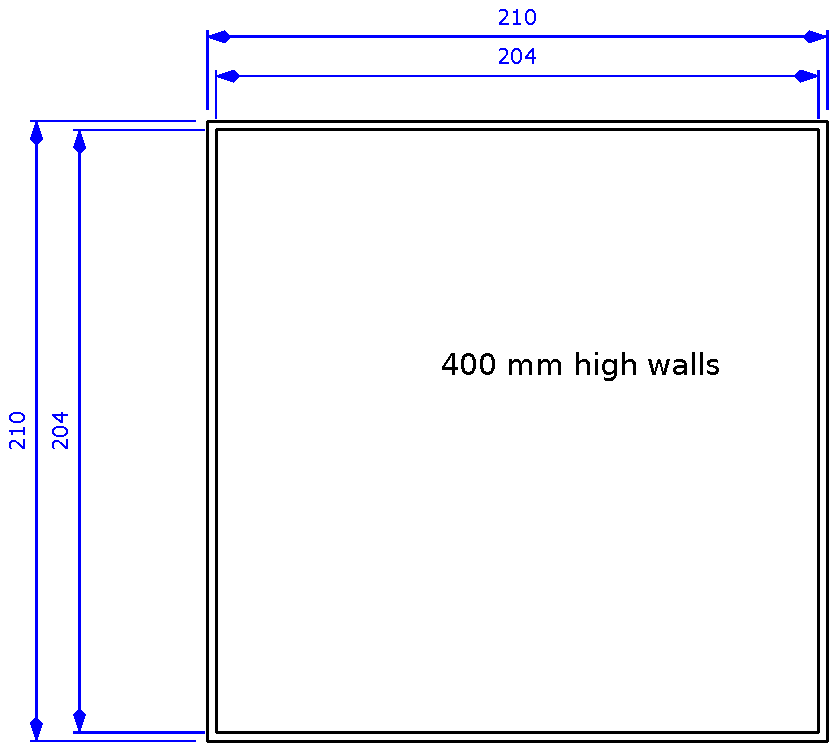
\includegraphics[scale=1]{RBR_cover}}  
  \caption{Blueprint of the RBR cover in scale 1:2}
  \label{fig:appendix-blueprint-rbr-cover}
    
\end{figure}
\begin{figure}[htbp]
  \centering
 \raisebox{-\height}{ 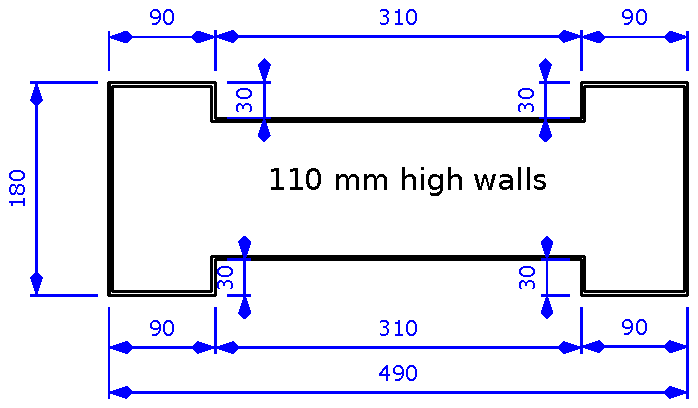
\includegraphics[scale=1]{Electric_cover}}
  \caption{Blueprint of the electric cover in scale 1:5}
  \label{fig:appendix-blueprint-electronic-cover}
    
\end{figure}
\section{Specification of requirements}
.\todo{Jesper}
\label{kravspec}
%%% Local Variables: 
%%% mode: latex
%%% TeX-master: "document"
%%% End: 
